\documentclass[10pt,conference]{IEEEtran}
\usepackage{amsmath,amssymb,booktabs,array,cite}
\usepackage[hidelinks]{hyperref}
\usepackage{url,tikz,balance}
\usetikzlibrary{arrows.meta,positioning}
\hypersetup{pdftitle={Recovery-Set Contracts for Cryptographic Storage Migration},pdfauthor={Ishan Teredesai and Tushar Rahangdale}}
\begin{document}
\title{Recovery-Set Contracts for Cryptographic Storage Migration}
\author{\IEEEauthorblockN{Ishan Teredesai \qquad Tushar Rahangdale}
\IEEEauthorblockA{Department of Information Technology\\
Yeshwantrao Chavan College of Engineering, Nagpur, India\\
teredesaishan@gmail.com \qquad tusharrahangadle@gmail.com}}
\maketitle
\begin{abstract}
Motivated by post-quantum migration, we study an algorithm-independent lifecycle problem: preserving the dependencies required to restore retained encrypted data. We specify an executable retirement contract distinguishing committed records, retained snapshots, and prepared work, together with a separate contract for approved-profile coverage. Eighteen bounded model configurations expose failures when retirement inspects intended updates or live records alone. A SQLite/AES-GCM harness reproduces those mechanisms in 126 deterministic cases, including 108 process terminations. We then challenge an unserialized implementation of the full recovery-set rule using two workers and four controlled schedules. Late dependency creation causes live restoration to fail in 12 of 24 unlocked cases. A cooperative lock covering dependency admission/publication and the complete retirement check/delete operation preserves restoration in all 24 protected cases; stale requests are rejected when their key has already been retired. These are selected case outcomes, not reliability estimates or a post-quantum security result. We contribute executable predicates, observed counterexample traces, a local synchronization experiment, and an illustrative acceptance case for migration tooling in critical systems.
\end{abstract}
\begin{IEEEkeywords}
cryptographic migration, key retirement, backup recovery, concurrency, software assurance
\end{IEEEkeywords}

\section{Introduction and Related Work}
Critical services must retain access to historical data while changing the cryptography that protects it. NIST storage guidance includes encryption keys and dependent key-management services in recovery planning~\cite{storage}. A hospital restoring an older patient-record snapshot after an incident therefore needs more than a working current encryption path. This is an illustrative requirement; we use synthetic data and evaluate no hospital deployment.

Post-quantum migration motivates the problem. ML-KEM standardizes a post-quantum key-establishment primitive~\cite{fips203}, while NIST's crypto-agility guidance addresses replacing cryptography while preserving operations~\cite{agility}. Our artifact evaluates algorithm-independent key-lifecycle dependencies. It uses AES-GCM wrapping-key epochs, without implementing ML-KEM, a hybrid KEM, or quantum entropy. In an envelope design, changing protection of a data encryption key (DEK) need not rewrite the bulk ciphertext, but retained envelopes may depend on earlier keys.

Key retention and crash consistency are established concerns. Key-management guidance covers inventories, backup, recovery, and destruction~\cite{keymgmt}. AWS KMS retains earlier AWS-generated key material for decryption~\cite{aws}; MongoDB documents rewrapping and warns against deleting keys still in use~\cite{mongo}. Pillai et al. analyze how application crash consistency depends on filesystem persistence behavior~\cite{pillai}. Table~\ref{tab:related} distinguishes these sources from our narrower artifact. We infer no missing product feature from silence in documentation and do not evaluate these products as baselines.

\begin{table}[t]
\caption{Relationship to verified prior work; no feature-absence claims}
\label{tab:related}\centering
\begin{tabular}{@{}p{2.15cm}p{2.7cm}p{2.95cm}@{}}
\toprule
Category & Source provides & This artifact provides\\
\midrule
Guidance~\cite{storage,keymgmt} & Recovery and key-lifecycle requirements & Executable reference and profile predicates\\
Rotation systems~\cite{aws,mongo} & Documented retention and rewrapping behavior & Explicit retirement obligations and negative controls\\
Crash consistency~\cite{pillai} & Application persistence analysis & Key-retirement counterexamples, restores, and controlled races\\
\bottomrule
\end{tabular}
\end{table}

Our position is that migration completion must cover the declared recovery set. We contribute an executable retirement contract distinguishing committed live references, retained recovery references, and volatile prepared work. We separately specify reference availability and approved-profile coverage, and evaluate retirement under transaction interruption and snapshot retention. We further examine synchronization between dependency creation and retirement through controlled concurrent schedules. The contribution is a testable engineering contract and focused evidence, not a new cryptographic construction or discovery that backups need keys.

\section{Contracts and Transition Model}
\subsection{Boundary and assumptions}
The finite model contains a trusted controller, available key generations, committed live record envelopes, one retained full snapshot, and volatile prepared targets. A generation identifies key material and an abstract protection-profile label. Generation zero is labeled legacy and later generations target; these labels do not establish algorithm security. Key compromise, malicious metadata, KMS outages, decoder incompatibility, and side channels lie outside the model. Compromise response may conflict with preserving a restore point; that conflict requires an explicit recovery/retention decision.

\subsection{Reference availability and retirement}
Let $S=(a,L,B,P,K)$ contain active generation $a$, committed live references $L$, optional snapshot $B$, pending targets $P$ (or $\bot$), and available generations $K$. Define
\begin{align}
R(S)&=\{L_i\}\cup\{B_i:B\text{ present}\},\\
I_{\mathrm{ref}}(S)&:\quad R(S)\subseteq K.
\end{align}
This invariant establishes key-reference availability, not complete service recovery. Decoder compatibility, authorization, and actual backup integrity remain separate requirements. The recovery-set guard permits removing generation $k$ only if
\begin{equation}
k\ne a\ \land\ k\notin R(S)\ \land\ k\notin\{P_i:P_i\ne\bot\}.
\label{eq:guard}
\end{equation}
Pending targets are not retained recovery references and therefore are absent from $I_{\mathrm{ref}}$. The additional clause protects prepared work from losing its target key before commit. A scan and deletion must be serialized with operations that can introduce dependencies; checking the right set once is insufficient when that set can change.

\subsection{Approved-profile coverage}
For approved profiles $\Pi$, define a second inventory property:
\begin{equation}
I_{\mathrm{profile}}(S):\ \forall r\in R(S),\ \operatorname{profile}(r)\in\Pi.
\end{equation}
The experiment interprets this as $r>0$. Live records can meet that condition while a recoverable snapshot remains legacy. Retaining its key preserves availability but leaves profile migration incomplete. The guard provides safety, not eventual completion. Rewrapping present envelopes cannot reverse exposure of an earlier copy already captured by an adversary.

\subsection{Transitions, controls, and preservation}
Initially, live records and the snapshot reference generation zero, $K=\{0\}$, and no work is pending. Activation durably provisions the next generation before making it active. Prepare requires an available source key and selects the active target. Commit atomically publishes a prepared target if its key is available. Crash clears pending work. Snapshot copies committed references when no snapshot exists. Release removes a retained snapshot obligation.

Release represents an \emph{authorized retention decision}; authorization itself is not modeled. It does not migrate the released snapshot or prove that it acquired a target profile. Neither release nor removal from $K$ establishes physical erasure, which has distinct medium and adversary assumptions~\cite{deletion}. Retention requirements cannot be satisfied merely by omitting an inconvenient copy from the declared set.

We compare intent-only retirement, which substitutes pending targets for live references and ignores the snapshot; live-only retirement, which checks committed live references alone; and recovery-set retirement, which applies (\ref{eq:guard}). The first two are deliberately weak controls. Under serialized transitions, preservation is direct: activation adds a key; prepare/crash leave durable references unchanged; commit targets an available key; snapshot copies valid references; release removes obligations; and guarded retirement removes no referenced key. This is an argument about the abstraction, not a verified distributed implementation.

Breadth-first traversal runs to a fixed point for each combination of one, two, or three records, two or three generations, and three policies: eighteen configurations. It has no depth cutoff. Snapshot release/recreation may repeat; states are deduplicated. Ordinary content updates, multiple snapshots, and replication are excluded. Tests also check guarded successors of structurally valid small states, including unreachable states.

\section{Executed Evaluation}
\subsection{Bounded reference model}
Table~\ref{tab:model} reports the largest configuration. Across all six recovery-set configurations, exploration visits 1,890 states and generates 7,232 transitions with no missing live or snapshot key, counting each configuration separately. Yet 293 states in its largest configuration have target-labeled live references and a legacy snapshot. Reference availability therefore does not imply profile completion.

\begin{table}[t]
\caption{Three records, three generations. Failure columns count states, can overlap, and are not probabilities.}
\label{tab:model}\centering
\begin{tabular}{@{}lrrr@{}}
\toprule
Rule & States & Missing live key & Missing backup key\\
\midrule
Intent-only & 3,682 & 1,814 & 1,766\\
Live-only & 1,996 & 0 & 403\\
Recovery-set & 1,495 & 0 & 0\\
\bottomrule
\end{tabular}
\end{table}

Minimal counterexamples require one record and two generations. Activate 1, prepare a replacement, then retire 0 under intent-only: the committed record still needs 0, and a crash discards the replacement. Alternatively, commit before live-only retirement: the live record uses 1 but the snapshot still needs 0. Recovery-set retirement remains blocked while that declared snapshot requires 0.

\subsection{Transaction interruption and snapshot retention}
A synthetic harness uses SQLite 3.53.1, Python 3.12.14, and \texttt{cryptography} 50.0.2 on Linux x86-64. Each record has a fresh 256-bit DEK. AES-256-GCM protects payloads and wrapped DEKs with separate random 96-bit nonces and associated data binding record identity and version/epoch. A JSON key file, updated through file synchronization and atomic replacement, contains unprotected test keys: it is not a secure KMS. SQLite uses rollback journaling and \texttt{synchronous=FULL}; its SQL transaction does not include the separate key file~\cite{sqlite}.

Figure~\ref{fig:lifecycle} shows rotation with a retained pre-rotation snapshot. The controller prepares all envelopes, attempts retirement, updates records in one SQL transaction, commits, and attempts retirement again. Six checkpoints terminate a child with \texttt{os.\_exit(93)}: after provisioning, preparation, first retirement, SQL updates before commit, commit, and final retirement. A seventh case completes normally. The parent reopens both copies and verifies recovered plaintext byte-for-byte.

\begin{figure}[t]
\centering
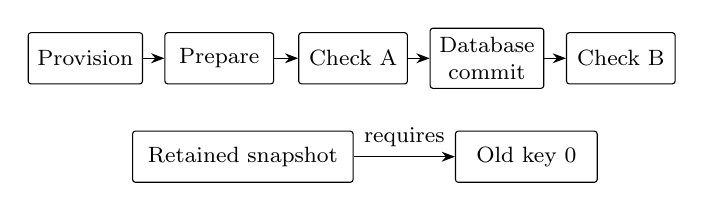
\begin{tikzpicture}[font=\footnotesize,box/.style={draw,rounded corners=1pt,align=center,minimum width=1.38cm,minimum height=.65cm},>=Stealth]
\node[box] (prov) at (0,0) {Provision};
\node[box] (prep) at (1.7,0) {Prepare};
\node[box] (first) at (3.4,0) {Check A};
\node[box] (commit) at (5.1,0) {Database\\commit};
\node[box] (last) at (6.8,0) {Check B};
\draw[->] (prov)--(prep); \draw[->] (prep)--(first);
\draw[->] (first)--(commit); \draw[->] (commit)--(last);
\node[box,minimum width=2.8cm] (snap) at (2,-1.25) {Retained snapshot};
\node[box,minimum width=1.8cm] (key) at (5.6,-1.25) {Old key 0};
\draw[->] (snap)--node[above]{requires} (key);
\end{tikzpicture}
\caption{Interruption harness. A: intent-only can retire the committed live key before commit. B: live-only can retire the snapshot's key after commit. The snapshot dependency persists across the entire rotation.}
\label{fig:lifecycle}
\end{figure}

One and eight records at 512 B, 16 KiB, and 256 KiB yield six datasets. Three rules and seven cases give 126 runs, including 108 process terminations. Each configuration runs once; no timings are measured. The host and filesystem remain running. Table~\ref{tab:crash} gives observed outcomes. Failures are missing wrapping keys; authentication errors, wrong row counts, or mismatched bytes abort the experiment. Intent-only fails live restoration at two cuts and backup restoration at five cut/completion points. Live-only fails backup restoration after final retirement and normal completion. Recovery-set retains the snapshot's key and restores both copies in all 42 cases.

\begin{table}[t]
\caption{Interruption harness: 42 deterministic cases per rule. Failure columns overlap; counts are coverage outcomes, not reliability estimates.}
\label{tab:crash}\centering
\begin{tabular}{@{}lrrr@{}}
\toprule
Rule & Live failure & Backup failure & Both restored\\
\midrule
Intent-only & 12 & 30 & 12\\
Live-only & 0 & 12 & 30\\
Recovery-set & 0 & 0 & 42\\
\bottomrule
\end{tabular}
\end{table}

\subsection{Challenging the guard with concurrent admission}
The earlier experiments assume serialized steps. We challenge an implementation of the \emph{full} recovery-set guard using two spawned workers: one checks/removes key 0; the other prepares and commits envelopes referencing 0. Initially, live records and the snapshot reference 1, active generation is 1, both keys exist, and no references are pending. Retirement of 0 is initially permitted.

The writer carries a previously selected generation choice, representing a delayed request or import. This admission operation extends the finite model's forward-only prepare step: it permits an inactive target while its key remains available. It deliberately tests a new dependency after a scan; it does not pretend that already registered pending work was absent. A current-generation-only deployment could reject such requests but must enforce that admission policy consistently.

Both implementations scan live records, the snapshot, and registered pending targets. The unlocked version separates that scan from deletion. The protected version uses one cooperative exclusive \texttt{fcntl.flock} on a stable local lock-file inode. The retirer holds it from the full scan through deletion. The writer holds the same lock across target-key availability validation, pin registration, preparation, database commit, and pin removal. Publication and pin removal share one SQL transaction. Merely locking deletion leaves the stale-scan gap open. Activation and snapshot changes are disabled during these trials; enabling them requires including them in the synchronization protocol.

The parent uses IPC gates to request four schedules without sleep-based ordering: (1) check, prepare, commit, delete; (2) check, prepare, delete, commit; (3) prepare, check, commit, delete; and (4) check, delete, prepare. A nonblocking lock attempt records contention; the holder finishes before the blocked operation is retried. Thus the protected implementation prevents the requested unsafe interleaving rather than executing it unchanged. Durable references and actual decryptions determine outcomes; no expected-result function supplies them.

\begin{table}[t]
\caption{Concurrent admission: six datasets per schedule and implementation (48 cases). L/B counts failed live/backup restores, not failure probabilities.}
\label{tab:concurrency}\centering
\begin{tabular}{@{}p{2.8cm}rrp{2.1cm}@{}}
\toprule
Requested schedule & \shortstack{Unlocked\\L/B} & \shortstack{Locked\\L/B} & Locked writer outcome\\
\midrule
Commit in scan/delete gap & 6/0 & 0/0 & 6 rejected\\
Prepare in scan/delete gap & 6/0 & 0/0 & 6 rejected\\
Writer prepares first & 0/0 & 0/0 & 6 committed\\
Retirement finishes first & 0/0 & 0/0 & 6 rejected\\
\bottomrule
\end{tabular}
\end{table}

Four schedules, two implementations, and six datasets give 48 cases. Table~\ref{tab:concurrency} reports observations. The unlocked version fails live restoration in 12/24 cases. In schedule 2, the scan sees no dependency on 0; the writer registers a pin; deletion uses the stale decision; commit publishes an envelope whose key is unavailable. When the pin precedes the scan (schedule 3), the guard sees it and denies retirement even without the lock.

All 24 protected cases restore live data and the snapshot. In the gap schedules, the writer encounters the held lock and is later rejected because retirement removed its key. With the writer first, retirement encounters the lock, retries after commit, sees the live reference, and retains the key. Schedule 4 rejects an unavailable target in both implementations. This connects the predicate to a local synchronization mechanism for selected admission schedules. It is not exhaustive concurrency coverage or a distributed lock/crash-recovery protocol. The concurrent trial's pending registry is a SQLite table; workers do not crash during these schedules.

\section{Illustrative Acceptance Case for Critical Systems}
Consider a hospital storage migration with retained incident-recovery snapshots. Table~\ref{tab:acceptance} separates illustrative deployment obligations from artifact evidence. The hypothetical hospital supplies context, not an industrial evaluation. A reference invariant cannot substitute for restoring a complete service with its decoder and authorization dependencies.

\begin{table}[t]
\caption{Illustrative acceptance case; deployment evidence remains required}
\label{tab:acceptance}\centering
\begin{tabular}{@{}p{1.8cm}p{3.1cm}p{2.9cm}@{}}
\toprule
Obligation & Required deployment evidence & Artifact coverage\\
\midrule
Recovery set & Manifest of retained copies and dependencies & One live set and one snapshot\\
Reference availability & Retirement decision using current references & Bounded predicate; local key checks\\
Profile coverage & Separate legacy-copy inventory/report & Abstract generation labels only\\
Restore capability & Restore declared data with actual decoder and authorization & Exact synthetic plaintext restores\\
Safe retirement & Dependency changes cannot race with deletion & Two cooperative local workers; four schedules\\
\bottomrule
\end{tabular}
\end{table}

Retention expiry must be authorized separately from migration. A legacy snapshot can be kept with its key, migrated through an approved copy-and-verify procedure, or released only when policy permits. Keeping it may indefinitely block retirement and profile completion. Deployments should report live coverage, retained-copy coverage, and blocked retirements separately, and validate the oldest retained restore point. Inventory size, snapshot chains, worker counts, KMS availability, recovery time, and lock contention remain evaluation dimensions; this study measures none of their costs.

\balance
\section{Limitations}
The finite model bounds records and generations, assumes complete inventories, and excludes ordinary content changes and replicas. The concurrent experiment adds stale-generation admission, so it is not an implementation proof of the closed model. Its advisory lock requires every relevant actor to cooperate; bypassing processes, remote KMS transactions, multiple lock domains, and worker failure during pin ownership need additional protocols. We test selected schedules, not all interleavings.

Process termination is not power loss; filesystem guarantees remain relevant~\cite{pillai}. Tiny synthetic datasets in one environment establish no throughput, scaling, or reliability estimate. Neither profile labels nor these tests establish confidentiality, hybrid-combiner security, secure erasure, or post-quantum protection. KEM integration requires separate protocol and implementation analysis~\cite{kem}. Nine regression tests and the raw traces support the stated artifact behavior, not production certification.

\section{Conclusion}
Retirement needs both a complete dependency predicate and synchronization with dependency creation. Our model separates reference availability from profile coverage; executed harnesses expose transaction, snapshot, and stale-scan failures. A shared local lock preserves restoration in the selected concurrent cases. These contracts and acceptance obligations provide a focused basis for evaluating migration tooling in critical systems.

\section*{Data and Code Availability}
Source, raw outcomes, event traces, environment manifests, tests, and LaTeX/PDF files are packaged with the supplement and maintained at \url{https://github.com/titcsl/storage-recovery-contracts}. The repository is private and requires access; the accompanying ZIP provides the same evidence for transfer through the venue's permitted artifact mechanism. The main paper is self-contained.

\section*{Acknowledgment}
OpenAI ChatGPT assisted with the abstract, Sections I--VI, tables and diagram, model formulation, experiment and validation code, revision, and reference checking. Reported results were obtained by executing the supplied programs.

\begin{thebibliography}{10}
\bibitem{storage} R. Chandramouli and D. Pinhas, \emph{Security Guidelines for Storage Infrastructure}, NIST SP 800-209, Oct. 2020, sec. 4.8, doi: \href{https://doi.org/10.6028/NIST.SP.800-209}{10.6028/NIST.SP.800-209}.
\bibitem{fips203} NIST, \emph{Module-Lattice-Based Key-Encapsulation Mechanism Standard}, FIPS 203, Aug. 2024, doi: 10.6028/NIST.FIPS.203.
\bibitem{agility} E. Barker et al., \emph{Considerations for Achieving Crypto Agility: Strategies and Practices}, NIST CSWP 39upd1, Dec. 2025, updated June 2026, doi: 10.6028/NIST.CSWP.39-upd1.
\bibitem{keymgmt} E. Barker, \emph{Recommendation for Key Management: Part 1---General}, NIST SP 800-57 Part 1 Rev. 5, May 2020, doi: 10.6028/NIST.SP.800-57pt1r5.
\bibitem{aws} Amazon Web Services, ``Rotate AWS KMS keys,'' AWS KMS Developer Guide. Accessed: Nov. 7, 2026. [Online]. Available: \url{https://docs.aws.amazon.com/kms/latest/developerguide/rotate-keys.html}
\bibitem{mongo} MongoDB, ``Rotate and rewrap encryption keys,'' MongoDB Manual. Accessed: Nov. 7, 2026. [Online]. Available: \url{https://www.mongodb.com/docs/manual/core/queryable-encryption/fundamentals/manage-keys/}
\bibitem{pillai} T. S. Pillai, V. Chidambaram, R. Alagappan, S. Al-Kiswany, A. C. Arpaci-Dusseau, and R. H. Arpaci-Dusseau, ``All file systems are not created equal: On the complexity of crafting crash-consistent applications,'' in \emph{Proc. 11th USENIX Symp. Operating Systems Design and Implementation (OSDI)}, 2014, pp. 433--448. [Online]. Available: \url{https://www.usenix.org/conference/osdi14/technical-sessions/presentation/pillai}
\bibitem{deletion} J. Reardon, D. Basin, and S. \v{C}apkun, ``SoK: Secure data deletion,'' in \emph{Proc. IEEE Symp. Security and Privacy}, 2013, pp. 301--315, doi: \href{https://doi.org/10.1109/SP.2013.28}{10.1109/SP.2013.28}.
\bibitem{sqlite} SQLite, ``Atomic commit in SQLite.'' Accessed: Nov. 7, 2026. [Online]. Available: \url{https://sqlite.org/atomiccommit.html}
\bibitem{kem} G. Alagic et al., \emph{Recommendations for Key-Encapsulation Mechanisms}, NIST SP 800-227, Sept. 2025, doi: 10.6028/NIST.SP.800-227.
\end{thebibliography}
\end{document}
